\section{The Coupled System}

While studying physical behavior of systems, one can find frequently a system linked to others (one or more) where its description depends on the simultaneous description of the others. Therefore, an independent solution is impossible without the parallel solutions of the rest. Such systems are called coupled and the way they interact will determine the coupled system behavior.

This section describes how the fluid-structure coupling is usually treated in a FEM analysis, a topic that concerns us for understanding and solving the problem proposed: the coupling between vibrations of the enclosed air and the plates of a Colombian C-Bandola. Here also will be exposed two simple models of coupled oscillators proposed by Christensen and Vistisen in \cite{Christensen, Christensen3}, where the enclosed air in a guitar and its plates are represented each by an individual oscillator. Basically, the use of these two coupling models will be useful as reference for numerical models and also for numerical results which must reflect predictions of coupling models and will provide further understanding since extended bodies can be modelled.

\subsection{Fluid-structure coupling}

Dynamic fluid-structure interaction can be followed when the motion of the structure induces pressure changes on the fluid (which doesn't penetrate the structure) and produces fluctuating motions. As the fluid moves, the varying pressure field loads the structure and its motion is modified. Thus, the process starts again. Considering the dynamic equations form for structures and the Helmholtz equation for acoustic problems, the expressions for a fluid-structure coupling are reached through Galerkin's variational method ("the weak form") which is useful in finite element method formulation. The coupling is presented using a discrete form of the previous resulted terms.

The weak form for solids can be presented as
\begin{equation}
\int_{\Omega_s} \delta \mathbf{u^T}(\rho_s \ddot{\mathbf{u}}+\mu \dot{\mathbf{u}}+ \mathbf{S^TDSu}-\mathbf{b}) d\Omega - \int_{\Gamma} \delta \mathbf{u^T}\bar{\mathbf{t}} d\Gamma = 0, 
\label{WeakSolid}
\end{equation}
where $\mathbf{u}$ and $\delta \mathbf{u^T}$ are the displacement vector and its variation, the superscript $T$ denotes the transpose; $\dot{\mathbf{u}}$ and $\ddot{\mathbf{u}}$ are the first and second time derivative of displacement vector. $\rho_s$ is the density of the solid, $\mu$ a damping constant, $\mathbf{S}$ is a linear differential operator, $\mathbf{D}$ the elasticity matrix containing the material properties and $\bar{\mathbf{t}}$ is the surface traction defined as
\[
\bar{\mathbf{t}}=-p\mathbf{n_s}= p\mathbf{n}.
\]
Above equation takes a positive pressure in compression and the outward normal to the solid $n_s=-n$. The traction integral in Eq. \ref{WeakSolid} is now expressed as
\[
\int_{\Gamma_t} \delta \mathbf{u^T} \bar{\mathbf{t}} d\Gamma = \int_{\Gamma_t} \delta \mathbf{u^T n}p d\Gamma.
\]

Since the fluid is coupled with the motion of the structure, the acceleration of the fluid particle is equal to the acceleration of the structure in the region of contact. Considering this, the weak form for the acoustic wave is
\begin{equation}
\int_{\Omega_f} \biggr[\delta p \frac{1}{c^2}\frac{\partial^2p}{\partial t^2}+(\nabla \delta p)^T (\nabla p) \biggr] d\Omega + \int_{\Gamma_1} \delta p \rho_0 \mathbf{n^T} \ddot{\mathbf{u}} d\Gamma = 0,
\label{WeakFluid-Bcond1}
\end{equation}
where $p$ and $\delta p$ are the pressure and its variation, $c$ is the sound velocity in the fluid, $\rho_0$ is the fluid density in the hydrostatic state and $\nabla$ is the Gradient. $\Omega_f$ and $\Omega_s$ are the fluid and structure domain, and $\Gamma$ is the boundary part where boundary conditions must be specified. It can be observed that both weak forms for fluid and solid depend on a variable defined in the other coupled phenomenon. This indicates the mutual dependence, i.e., the coupling.\\

In Eq.\ref{WeakFluid-Bcond1} and Eq.\ref{WeakSolid}, pressure and displacement vectors $p$ and $u$ will be approximated to discretize the system. For this, a shape function is proposed in order to fix pressure and displacement values in a specific domain. This can be expressed as
\begin{eqnarray*}
p & \approx & \hat{p}= N_p\tilde{p}\\
u & \approx & \hat{u}= N_u\tilde{u},
\end{eqnarray*}
where $\tilde{p}$ and $\tilde{u}$ are the vectors of values for pressure and displacement at every point defined in the domain and $N_p$ and $N_u$ are appropriate shape matrices that fix the values at the points in the domain. \\

Discretization applied to fluid equation in Eq.\ref{WeakFluid-Bcond1} yields
\begin{equation}
S\ddot{\tilde{p}}+ H\tilde{p}+\rho_0 Q^T \ddot{\tilde{u}}+q = 0,
\label{DiscreteFluid}
\end{equation}
where $q$ is an included source term and
\begin{equation}
\left.
\begin{aligned}
S & = \int_\Omega N^T_p \frac{1}{c^2} N_p d\Omega \\ %\int_{\Gamma_3} N^T_p \frac{1}{g} N_p d\Gamma\\
%\tilde{C} & = \int_{\Gamma_4} N^T_p \frac{1}{c} N_p d\Gamma\\
H & = \int_\Omega (\nabla N_p)^T \nabla N_p d\Omega\\
Q & = \int_{\Gamma_t} N^T_u \mathbf{n} N_p d\Gamma
\end{aligned}
\right\}
\label{Qterm}
\end{equation}

Similarly, the discrete structural problem becomes
\begin{equation}
M\ddot{\tilde{u}}+C\dot{\tilde{u}}+K\tilde{u}-Q\tilde{p}+f=0,
\label{DiscreteSolid}
\end{equation}
where
\begin{eqnarray*}
M & = & \int_\Omega N^T_u \rho_s N_u d\Omega\\
C & = & \int_\Omega N^T_u \mu N_u d\Omega\\
K & = & \int_\Omega B^T D B d\Omega\\
q & = & -\int_\Omega N_u b d\Omega.
\end{eqnarray*}
$B= SN_u$ and $Q$ is identical to Eq. \ref{Qterm}.\\

If free vibrations are considered and all forces and damping terms are omitted, Eq.\ref{DiscreteFluid} and Eq.\ref{DiscreteSolid} can be written as
\[
\begin{bmatrix}
M & 0\\
\rho_0 Q^T & S
\end{bmatrix}
\begin{Bmatrix}
\ddot{\tilde{u}}\\ \ddot{\tilde{p}}
\end{Bmatrix}
+\begin{bmatrix}
K & -Q\\
0 & H
\end{bmatrix}
\begin{Bmatrix}
\tilde{u}\\ \tilde{p}
\end{Bmatrix} = 0
\]
This is the system of equations that represents our fluid-structure interaction problem. For an eigenvalue problem, it is observed that the system is not symmetric and standard eigenvalue extraction methods are not direct applicable. However, the system is positive semidefinite and it is physically clear that eigenvalues are real and free vibration modes exist.
 
\subsection{Simple model of coupled oscillators}

Modal coupling analysis at low resonances in a bandola can be performed by assuming a coupling model for resonance box. Reported works on the subject \cite{Rossing1, Meyer, Meyer2, Rossing, Rossing3, Christensen, Christensen3, Caldersmith1, Dickens1, Firth1} commonly start with the analysis of two  simple coupling models, each with two and three coupled oscillators respectively. For instance, Meyer, Rossing and Christensen \cite{Rossing1, Meyer, Christensen3} describe that three coupled oscillators: top plate, enclosed air and back plate, produce the first three modal frequencies of a classical guitar resonance box which correspond to combination modes. Considering works in \cite{Meyer2, Rossing3, Christensen}, these authors also reported that a model with two oscillators: top plate and enclosed air, will predict the first two resonances.\\

According to above ideas and taking in mind that guitars are the closest acoustical reference of bandolas, numerical models that reflect these coupled systems are proposed for modal coupling analysis. Thus, numerical solutions could describe dynamic behavior in the bandola at its first two or three resonances for each case.

\subsubsection{Coupling between top plate and enclosed air.}

Based on the model presented by Christensen and Vistisen in \cite{Christensen}, the coupling between top plate and enclosed air is presented on the basis of Newtonian equations of motion. The model consider the interaction of resonances of two oscillators: Helmholtz resonance and the fundamental top plate resonance. The air inside the cavity vibrates somehow like a Helmholtz resonator for the first mode. In this case, this resonator consist of an air piston in the sound hole, oscillating against the stiffness of the air in the cavity. The fundamental top plate mode in a guitar is characterized by symmetrical variation of amplitude over the lower bout of the guitar \cite{Jansson:GuitarModes}, hence, the model consider this fundamental resonance assuming a simple harmonic oscillator consisting of a plate mass and a piston area, together with a spring stiffness. The back plate is assumed rigid. Figure \ref{Top-Air} illustrates the model.

\begin{figure}[h]
\centering
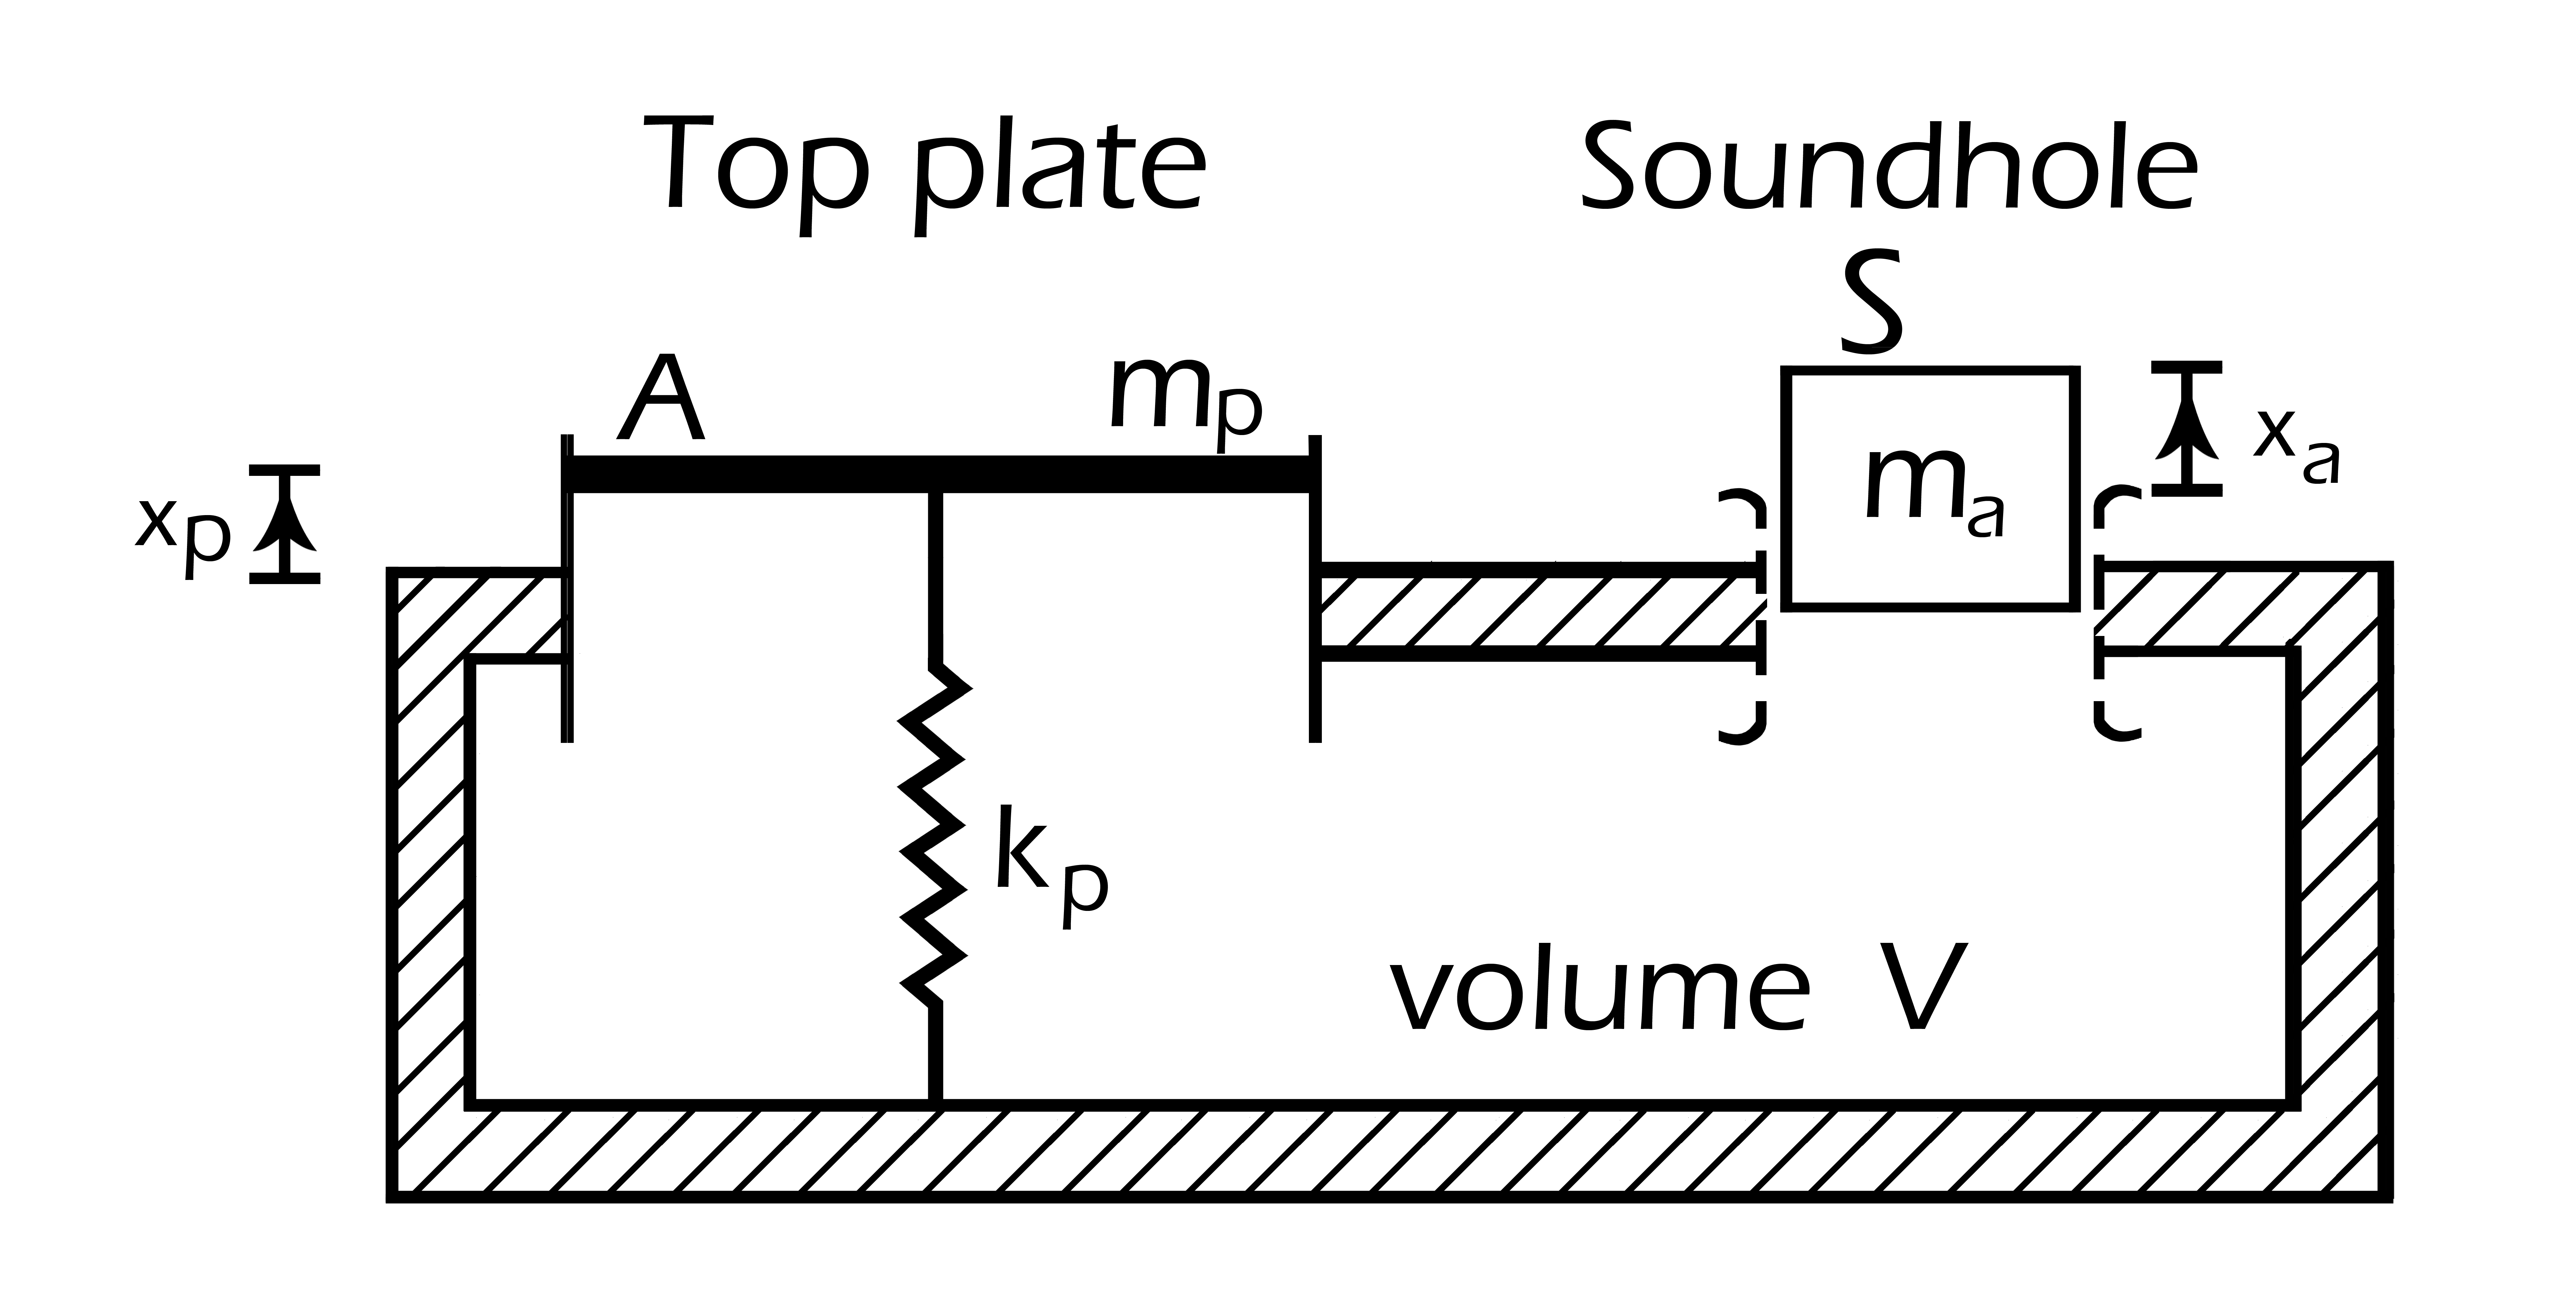
\includegraphics[height=2.5cm]{img/Top-Air.png}
\caption{Coupling model of resonance box of two oscillators presented by Christensen and Vistisen}
\label{Top-Air}
\end{figure}


Equations of motion for the system of two coupled oscillators are:
\begin{eqnarray}
m_{p}\ddot{x}_p & = & - k_p x_p  + A \Delta p
\label{EqPlate}\\
m_{a}\ddot{x}_a & = & S \Delta p,
\label{EqAir}
\end{eqnarray}
where $\Delta p  = - \mu \Delta V$, $\mu= c^2 \rho_a / V$, $\Delta V  =  A x_p + S x_a$ and
\begin{eqnarray*}
& x_p \quad  &\text{the displacement of top plate piston}\\
& x_a \quad &\text{the displacement of air piston}\\
& m_p \quad &\text{the plate mass}\\
& m_a \quad &\text{the air piston mass}\\
& k_p \quad &\text{the spring stiffness}\\
& A \quad &\text{the equivalent piston area of top plate}\\
& S \quad &\text{the area of soundhole}\\
& c \quad &\text{the sound velocity in air}\\
& \rho_a \quad &\text{the density of air}\\
& V \quad &\text{the cavity volume}
\end{eqnarray*}
Assuming $x_p=A_p e^{i\omega_p t}$ and $x_a=A_a e^{i\omega_h t}$ in E.q.\ref{EqPlate} and E.q.\ref{EqAir} and using a matrix-vector form, solution of the system is found for the characteristic polynomial:
\begin{equation}
\left( \omega^2 - \frac{k_p + \mu A^2}{m_p} \right) \left( \omega^2 - \frac{\mu S^2}{m_a} \right) - \frac{(\mu SA)^2}{m_p m_a} =0.
\label{2Poly}
\end{equation}
It can be noted from E.q.\ref{EqPlate} and E.q.\ref{EqAir} that resonance frequencies for both separate systems (plate and piston air) $\omega_p$ and $\omega_h$ respectively, are:
\begin{eqnarray*}
\omega^2_p = \frac{k_p + \mu A^2}{m_p}\\
\omega^2_h = \frac{\mu S^2}{m_a},
\end{eqnarray*}
with $\omega^4_{ph}=(\mu SA)^2/m_p m_a$ as a coupling frequency, E.q.\ref{2Poly} yields:
\begin{equation}
(\omega^2 - \omega^2_p)(\omega^2 - \omega^2_h)- \omega^4_{ph} =0,
\end{equation}
An important relation can be given by summing the roots of this system of two oscillators:
\begin{equation}
\omega_{1}^2 + \omega_{2}^2 = \omega^2_p + \omega^2_h.
\label{Combination2}
\end{equation}
Above equation says that square sum of the resonance frequencies in the coupled system equals the square sum of resonances frequencies in the uncoupled system.\\

The model presented by Christensen and Vistinsen is validated through mobility and sound radiation measurements that confirm the great approach to guitar dynamic behavior at the first two resonances. As they mentioned \cite{Christensen}, "the only condition for establishment of a coupling is that the Helmholtz resonance is present and that the vibration of the top plate (plus back plate eventually) generates a net volume displacement". Therefore, the behavior of bandola at the first two resonances is assumed to be described by this model, and the use of FEM will give a wider scope since it considers an extended body which allows detailed information at every point.

\subsubsection{Coupling between top plate, enclosed air and back plate.}

The influence of the back plate is modelled by introducing another piston with effective area $B$ and mass $m_b$ which acts against a spring of stiffness $k_b$, as described by Christensen \cite{Christensen3}. Motion of any piston causes pressure changes inside the cavity and will affect the motion of the other two pistons. The system of coupled pistons is given in Figure \ref{Top-Back-Air}.

\begin{figure}[h]
\centering
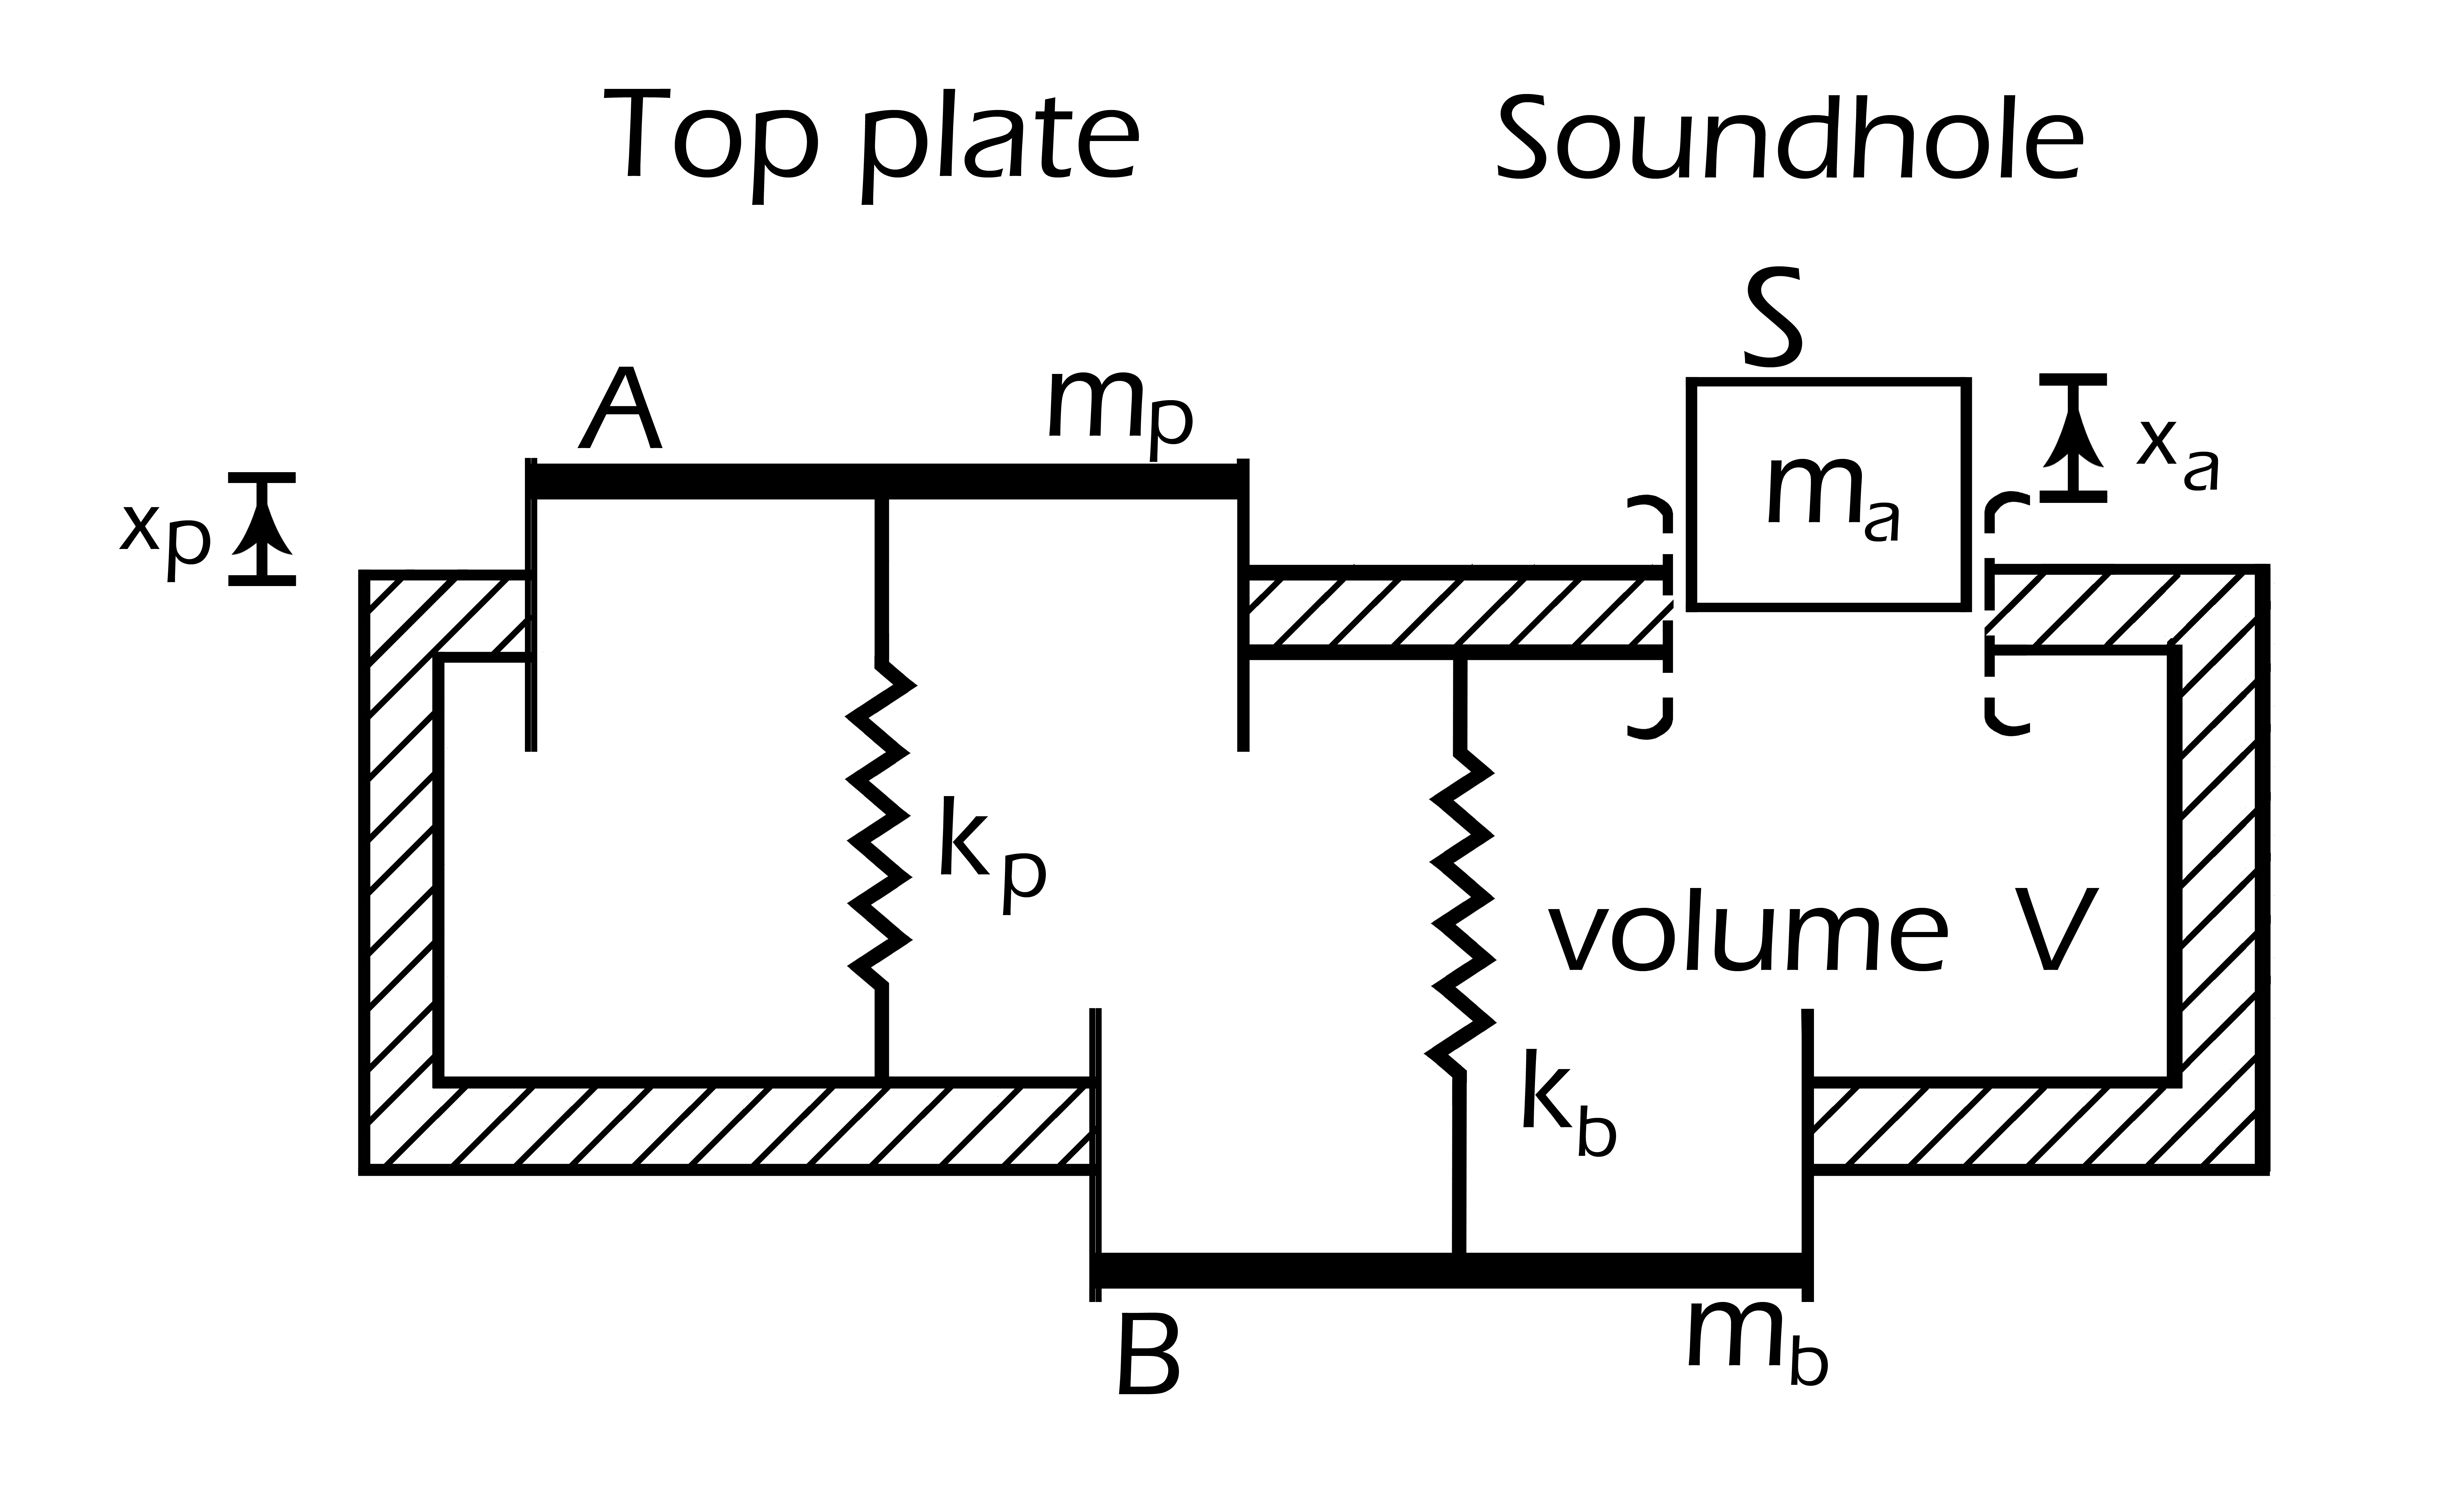
\includegraphics[height=3cm]{img/Top-Back-Air.png}
\caption{Coupling model of resonance box of three oscillators presented by Christensen}
\label{Top-Back-Air}
\end{figure}

The equations of motion for the three pistons in the coupled system are:
\begin{eqnarray}
m_{p}\ddot{x}_p & = & - k_p x_p  + A \Delta p
\label{EqPlate1}\\
m_{a}\ddot{x}_a & = & S \Delta p
\label{EqAir1}\\
m_{b}\ddot{x}_b & = & - k_b x_b  + B \Delta p,
\label{EqBack1}
\end{eqnarray}
where $x_b$ is the displacement of back plate piston.
$\Delta p$, as before, is the pressure change in the cavity resulting from movements of the pistons. Thus,
\begin{eqnarray*}
\Delta p & = & -\mu \Delta V\\
\Delta V & = & A x_p + S x_a + B x_b
\end{eqnarray*}
Again, it is assumed $x_p=A_p e^{i\omega_p t}$, $x_a=A_a e^{i\omega_h t}$ and $x_b=A_b e^{i\omega_b t}$ for equations in Eqs.\ref{EqPlate1}-\ref{EqBack1}. Thus, it can be identified, as in the model of two oscillators, the resonance frequencies of separate systems and the coupling frequencies.\\

Using the matrix-vector form, it can be found the characteristic polynomial and its roots. It is shown, by summing the roots, that it is also held the relation where the square sum of coupled resonance frequencies is equal to the sum of uncoupled resonance frequencies. Thus,
\begin{equation}
\omega_{1}^2 + \omega_{2}^2 + \omega_{3}^2 = \omega^2_p + \omega^2_h + \omega^2_b.
\label{Combination3}
\end{equation}
Meyer \cite{Meyer2} was the first one to give a detailed technical description for the three-oscillators system. He showed that the effect of back plate is to lower $\omega_1$ and $\omega_2$ and to split $\omega_2$ in two resonances yielding $\omega_3$.\\

This model is used for description of bandola behavior at the first three resonances, where again the use of FEM will give a wider scope. It was observed that coupled modes are expressed in terms of uncoupled modes, so, numerical models for separate oscillators (of each model) are proposed for analysis in order to appreciate, through comparison, their participation in coupled modes.\\

An useful detail for analysis can be noted in coupling frequency terms. These terms are ratios of the piston areas and the effective mass of oscillating pistons, with more terms for the case of three oscillators. It can be infer of this fact that a weak or strong coupling will depend on this ratios.